\subsection{逻辑切分}\label{logicaldivisionsection}

\noindent 本节定义布局（layout）的{\bf 逻辑切分}（logical division）。作为一个动机示例，考虑布局

\bigskip

\begin{centering}
    
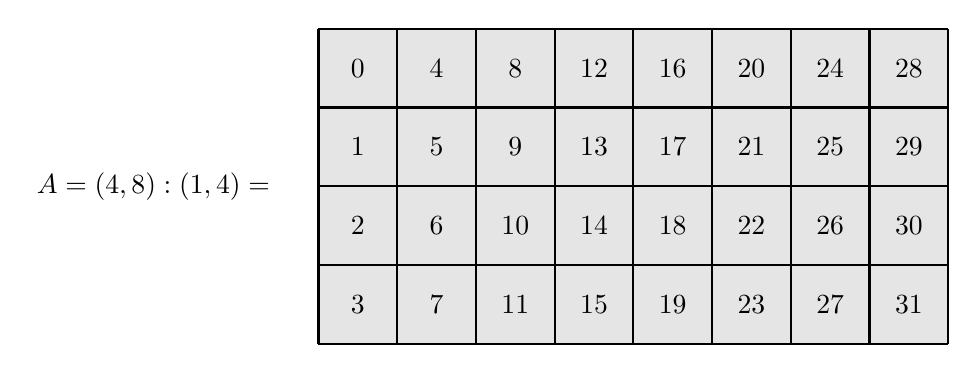
\begin{tikzpicture}[x={(0cm,-1cm)},y={(1cm,0cm)},every node/.style={minimum size=1cm, outer sep=0pt}]

\node[fill=gray!20] at (0,0) {0};
\node[fill=gray!20] at (0,1) {4};
\node[fill=gray!20] at (0,2) {8};
\node[fill=gray!20] at (0,3) {12};
\node[fill=gray!20] at (0,4) {16};
\node[fill=gray!20] at (0,5) {20};
\node[fill=gray!20] at (0,6) {24};
\node[fill=gray!20] at (0,7) {28};
\node[fill=gray!20] at (1,0) {1};
\node[fill=gray!20] at (1,1) {5};
\node[fill=gray!20] at (1,2) {9};
\node[fill=gray!20] at (1,3) {13};
\node[fill=gray!20] at (1,4) {17};
\node[fill=gray!20] at (1,5) {21};
\node[fill=gray!20] at (1,6) {25};
\node[fill=gray!20] at (1,7) {29};
\node[fill=gray!20] at (2,0) {2};
\node[fill=gray!20] at (2,1) {6};
\node[fill=gray!20] at (2,2) {10};
\node[fill=gray!20] at (2,3) {14};
\node[fill=gray!20] at (2,4) {18};
\node[fill=gray!20] at (2,5) {22};
\node[fill=gray!20] at (2,6) {26};
\node[fill=gray!20] at (2,7) {30};
\node[fill=gray!20] at (3,0) {3};
\node[fill=gray!20] at (3,1) {7};
\node[fill=gray!20] at (3,2) {11};
\node[fill=gray!20] at (3,3) {15};
\node[fill=gray!20] at (3,4) {19};
\node[fill=gray!20] at (3,5) {23};
\node[fill=gray!20] at (3,6) {27};
\node[fill=gray!20] at (3,7) {31};
\draw[color=black,thick,shift={(-0.5,-0.5)}] (0,0) grid (4,8);

\node[anchor=east] at (1.5,-1) {$A = (4,8):(1,4) = $};
\end{tikzpicture}

\end{centering} 

\bigskip

\noindent 出于各种目的，我们可能希望对布局 $A$ 进行{\it 铺砌}（tile）。例如，下面给出了用几种不同布局 $B$ 对 $A$ 所作的铺砌（tiling）。

\bigskip


\begin{centering}

\begin{tikzpicture}[x={(0cm,-1cm)},y={(1cm,0cm)},every node/.style={minimum size=1cm, outer sep=0pt}]

\node[fill=colorx1!60] at (0,0) {0};
\node[fill=colorx1!60] at (0,1) {4};
\node[fill=colorx3!60] at (0,2) {8};
\node[fill=colorx3!60] at (0,3) {12};
\node[fill=colorx5!60] at (0,4) {16};
\node[fill=colorx5!60] at (0,5) {20};
\node[fill=colorx7!60] at (0,6) {24};
\node[fill=colorx7!60] at (0,7) {28};
\node[fill=colorx1!60] at (1,0) {1};
\node[fill=colorx1!60] at (1,1) {5};
\node[fill=colorx3!60] at (1,2) {9};
\node[fill=colorx3!60] at (1,3) {13};
\node[fill=colorx5!60] at (1,4) {17};
\node[fill=colorx5!60] at (1,5) {21};
\node[fill=colorx7!60] at (1,6) {25};
\node[fill=colorx7!60] at (1,7) {29};
\node[fill=colorx2!60] at (2,0) {2};
\node[fill=colorx2!60] at (2,1) {6};
\node[fill=colorx4!60] at (2,2) {10};
\node[fill=colorx4!60] at (2,3) {14};
\node[fill=colorx6!60] at (2,4) {18};
\node[fill=colorx6!60] at (2,5) {22};
\node[fill=colorx8!60] at (2,6) {26};
\node[fill=colorx8!60] at (2,7) {30};
\node[fill=colorx2!60] at (3,0) {3};
\node[fill=colorx2!60] at (3,1) {7};
\node[fill=colorx4!60] at (3,2) {11};
\node[fill=colorx4!60] at (3,3) {15};
\node[fill=colorx6!60] at (3,4) {19};
\node[fill=colorx6!60] at (3,5) {23};
\node[fill=colorx8!60] at (3,6) {27};
\node[fill=colorx8!60] at (3,7) {31};
\draw[color=black,thick,shift={(-0.5,-0.5)}] (0,0) grid (4,8);

\node at (1.5,-1) {$A = $};
\node at (1.5,9) {$B = $};

\node[fill=gray!20] at (1,10) {0};
\node[fill=gray!20] at (2,10) {1};
\node[fill=gray!20] at (1,11) {4};
\node[fill=gray!20] at (2,11) {5};
\draw[color=black,thick,shift={(-0.5,-0.5)}] (1,10) grid (3,12);

\node[fill=colorx1!60] at (5,0) {0};
\node[fill=colorx1!60] at (5,1) {4};
\node[fill=colorx1!60] at (5,2) {8};
\node[fill=colorx1!60] at (5,3) {12};
\node[fill=colorx5!60] at (5,4) {16};
\node[fill=colorx5!60] at (5,5) {20};
\node[fill=colorx5!60] at (5,6) {24};
\node[fill=colorx5!60] at (5,7) {28};
\node[fill=colorx3!60] at (6,0) {1};
\node[fill=colorx3!60] at (6,1) {5};
\node[fill=colorx3!60] at (6,2) {9};
\node[fill=colorx3!60] at (6,3) {13};
\node[fill=colorx7!60] at (6,4) {17};
\node[fill=colorx7!60] at (6,5) {21};
\node[fill=colorx7!60] at (6,6) {25};
\node[fill=colorx7!60] at (6,7) {29};
\node[fill=colorx1!60] at (7,0) {2};
\node[fill=colorx1!60] at (7,1) {6};
\node[fill=colorx1!60] at (7,2) {10};
\node[fill=colorx1!60] at (7,3) {14};
\node[fill=colorx5!60] at (7,4) {18};
\node[fill=colorx5!60] at (7,5) {22};
\node[fill=colorx5!60] at (7,6) {26};
\node[fill=colorx5!60] at (7,7) {30};
\node[fill=colorx3!60] at (8,0) {3};
\node[fill=colorx3!60] at (8,1) {7};
\node[fill=colorx3!60] at (8,2) {11};
\node[fill=colorx3!60] at (8,3) {15};
\node[fill=colorx7!60] at (8,4) {19};
\node[fill=colorx7!60] at (8,5) {23};
\node[fill=colorx7!60] at (8,6) {27};
\node[fill=colorx7!60] at (8,7) {31};
\draw[color=black,thick,shift={(-0.5,-0.5)}] (5,0) grid (9,8);

\node at (6.5,-1) {$A = $};
\node at (6.5,9) {$B = $};

\node[fill=gray!20] at (6,10) {0};
\node[fill=gray!20] at (7,10) {2};
\node[fill=gray!20] at (6,11) {4};
\node[fill=gray!20] at (7,11) {6};
\node[fill=gray!20] at (6,12) {8};
\node[fill=gray!20] at (7,12) {10};
\node[fill=gray!20] at (6,13) {12};
\node[fill=gray!20] at (7,13) {14};
\draw[color=black,thick,shift={(-0.5,-0.5)}] (6,10) grid (8,14);

\node[fill=colorx1!60] at (10,0) {0};
\node[fill=colorx1!60] at (10,1) {4};
\node[fill=colorx3!60] at (10,2) {8};
\node[fill=colorx3!60] at (10,3) {12};
\node[fill=colorx1!60] at (10,4) {16};
\node[fill=colorx1!60] at (10,5) {20};
\node[fill=colorx3!60] at (10,6) {24};
\node[fill=colorx3!60] at (10,7) {28};
\node[fill=colorx5!60] at (11,0) {1};
\node[fill=colorx5!60] at (11,1) {5};
\node[fill=colorx7!60] at (11,2) {9};
\node[fill=colorx7!60] at (11,3) {13};
\node[fill=colorx5!60] at (11,4) {17};
\node[fill=colorx5!60] at (11,5) {21};
\node[fill=colorx7!60] at (11,6) {25};
\node[fill=colorx7!60] at (11,7) {29};
\node[fill=colorx1!60] at (12,0) {2};
\node[fill=colorx1!60] at (12,1) {6};
\node[fill=colorx3!60] at (12,2) {10};
\node[fill=colorx3!60] at (12,3) {14};
\node[fill=colorx1!60] at (12,4) {18};
\node[fill=colorx1!60] at (12,5) {22};
\node[fill=colorx3!60] at (12,6) {26};
\node[fill=colorx3!60] at (12,7) {30};
\node[fill=colorx5!60] at (13,0) {3};
\node[fill=colorx5!60] at (13,1) {7};
\node[fill=colorx7!60] at (13,2) {11};
\node[fill=colorx7!60] at (13,3) {15};
\node[fill=colorx5!60] at (13,4) {19};
\node[fill=colorx5!60] at (13,5) {23};
\node[fill=colorx7!60] at (13,6) {27};
\node[fill=colorx7!60] at (13,7) {31};
\draw[color=black,thick,shift={(-0.5,-0.5)}] (10,0) grid (14,8);

\node at (11.5,-1) {$A = $};
\node at (11.5,9) {$B = $};

\node[fill=gray!20] at (11,10) {0};
\node[fill=gray!20] at (12,10) {2};
\node[fill=gray!20] at (11,11) {4};
\node[fill=gray!20] at (12,11) {6};
\node[fill=gray!20] at (11,12) {16};
\node[fill=gray!20] at (12,12) {18};
\node[fill=gray!20] at (11,13) {20};
\node[fill=gray!20] at (12,13) {22};
\draw[color=black,thick,shift={(-0.5,-0.5)}] (11,10) grid (13,14);
\end{tikzpicture}

\end{centering}


\bigskip 

在处理这类经过铺砌的布局时，我们希望能够用形如 $(\texttt{tile}\_\texttt{coordinate},\texttt{tile})$ 的坐标对布局进行索引，其中 $\texttt{tile}$ 指明我们正在操作的是哪一个瓦片（tile），而 $\texttt{tile}\_\texttt{coordinate}$ 指明所给瓦片内部的一个坐标。例如，若 $A$ 与 $B$ 的秩（rank）均为 $2$，我们便希望把 $((i,j),(k,\ell))$ 写作 $A$ 的第 $(k,\ell)$ 个瓦片中第 $(i,j)$ 个元素（entry）的索引。逻辑切分 $A \oslash B$ 正是为我们提供这一能力的布局。



\begin{definition}\label{definitionoflogicaldivide}
设 $A$ 与 $B$ 为布局，并设
\[B^c = \comp(B,\size(A))\]
为 $B$ 关于 $\size(A)$ 的补（complement）。则 $A$ 除以 $B$ 的{\it 逻辑切分}是布局
\begin{align*}
A \oslash B & = A \circ (B,B^c)\\
& = (A \circ B, A \circ B^c).
\end{align*}
\end{definition}


\begin{example}
    若 $A = (4,8):(1,4)$ 且 $B = (2,2):(1,4)$，则
    \[A \oslash B = ((2,2),(2,4)):((1,4),(2,8)),\]
    如下图所示。

    \bigskip


\begin{centering}
\begin{tikzpicture}[x={(0cm,-1cm)},y={(1cm,0cm)},every node/.style={minimum size=1cm, outer sep=0pt}]

\node[fill=colorx1!60] at (0,0) {0};
\node[fill=colorx1!60] at (0,1) {4};
\node[fill=colorx3!60] at (0,2) {8};
\node[fill=colorx3!60] at (0,3) {12};
\node[fill=colorx5!60] at (0,4) {16};
\node[fill=colorx5!60] at (0,5) {20};
\node[fill=colorx7!60] at (0,6) {24};
\node[fill=colorx7!60] at (0,7) {28};
\node[fill=colorx1!60] at (1,0) {1};
\node[fill=colorx1!60] at (1,1) {5};
\node[fill=colorx3!60] at (1,2) {9};
\node[fill=colorx3!60] at (1,3) {13};
\node[fill=colorx5!60] at (1,4) {17};
\node[fill=colorx5!60] at (1,5) {21};
\node[fill=colorx7!60] at (1,6) {25};
\node[fill=colorx7!60] at (1,7) {29};
\node[fill=colorx2!60] at (2,0) {2};
\node[fill=colorx2!60] at (2,1) {6};
\node[fill=colorx4!60] at (2,2) {10};
\node[fill=colorx4!60] at (2,3) {14};
\node[fill=colorx6!60] at (2,4) {18};
\node[fill=colorx6!60] at (2,5) {22};
\node[fill=colorx8!60] at (2,6) {26};
\node[fill=colorx8!60] at (2,7) {30};
\node[fill=colorx2!60] at (3,0) {3};
\node[fill=colorx2!60] at (3,1) {7};
\node[fill=colorx4!60] at (3,2) {11};
\node[fill=colorx4!60] at (3,3) {15};
\node[fill=colorx6!60] at (3,4) {19};
\node[fill=colorx6!60] at (3,5) {23};
\node[fill=colorx8!60] at (3,6) {27};
\node[fill=colorx8!60] at (3,7) {31};
\draw[color=black,thick,shift={(-0.5,-0.5)}] (0,0) grid (4,8);

\node[anchor = east] at (1.5,-1) {$A = $};
\node[anchor = east] at (1.5,9.5) {$B = $};

\node[fill=gray!5] at (1,10) {0};
\node[fill=gray!20] at (2,10) {1};
\node[fill=gray!40] at (1,11) {4};
\node[fill=gray!60] at (2,11) {5};
\draw[color=black,thick,shift={(-0.5,-0.5)}] (1,10) grid (3,12);
\end{tikzpicture}

\end{centering}

\vspace{0.2in}

\begin{centering}
\begin{tikzpicture}[x={(0cm,-1cm)},y={(1cm,0cm)},every node/.style={minimum size=1cm, outer sep=0pt}]

\node[fill=colorx1!10]       at (0,0) {0};
\node[fill=colorx2!10]       at (0,1) {2};
\node[fill=colorx3!10]      at (0,2) {8};
\node[fill=colorx4!10]      at (0,3) {10};
\node[fill=colorx5!10]  at (0,4) {16};
\node[fill=colorx6!10]  at (0,5) {18};
\node[fill=colorx7!10]        at (0,6) {24};
\node[fill=colorx8!10]        at (0,7) {26};

\node[fill=colorx1!25]       at (1,0) {1};
\node[fill=colorx2!25]       at (1,1) {3};
\node[fill=colorx3!25]      at (1,2) {9};
\node[fill=colorx4!25]      at (1,3) {11};
\node[fill=colorx5!25]  at (1,4) {17};
\node[fill=colorx6!25]  at (1,5) {19};
\node[fill=colorx7!25]        at (1,6) {25};
\node[fill=colorx8!25]        at (1,7) {27};

\node[fill=colorx1!40]       at (2,0) {4};
\node[fill=colorx2!40]       at (2,1) {6};
\node[fill=colorx3!40]      at (2,2) {12};
\node[fill=colorx4!40]      at (2,3) {14};
\node[fill=colorx5!40]  at (2,4) {20};
\node[fill=colorx6!40]  at (2,5) {22};
\node[fill=colorx7!40]        at (2,6) {28};
\node[fill=colorx8!40]        at (2,7) {30};

\node[fill=colorx1!60]       at (3,0) {5};
\node[fill=colorx2!60]       at (3,1) {7};
\node[fill=colorx3!60]      at (3,2) {13};
\node[fill=colorx4!60]      at (3,3) {15};
\node[fill=colorx5!60]  at (3,4) {21};
\node[fill=colorx6!60]  at (3,5) {23};
\node[fill=colorx7!60]       at (3,6) {29};
\node[fill=colorx8!60]       at (3,7) {31};
\draw[color=black,thick,shift={(-0.5,-0.5)}] (0,0) grid (4,8);

\node[anchor=east] at (1.5,-1) {$ A \oslash B = $};

\end{tikzpicture}

\end{centering}
\end{example}

\begin{remark}
    $A \oslash B$ 中每个元素的{\it 颜色}（color）表明它属于哪个瓦片，而 $A\oslash B$ 中每个元素的{\it 不透明度}（opacity）表明它代表该瓦片中的哪个元素。这正是 $A\oslash B$ 的每一列颜色相同、每一行不透明度相同的原因。
\end{remark}


\begin{example}
    若 $A = (4,8):(1,4)$ 且 $B = (2,2):(4,1)$，则
    \[A \oslash B = ((2,2),(2,4)):((4,1),(2,8)),\]
    如下图所示。

    \bigskip


\begin{centering}
\begin{tikzpicture}[x={(0cm,-1cm)},y={(1cm,0cm)},every node/.style={minimum size=1cm, outer sep=0pt}]

\node[fill=colorx1!60] at (0,0) {0};
\node[fill=colorx1!60] at (0,1) {4};
\node[fill=colorx3!60] at (0,2) {8};
\node[fill=colorx3!60] at (0,3) {12};
\node[fill=colorx5!60] at (0,4) {16};
\node[fill=colorx5!60] at (0,5) {20};
\node[fill=colorx7!60] at (0,6) {24};
\node[fill=colorx7!60] at (0,7) {28};
\node[fill=colorx1!60] at (1,0) {1};
\node[fill=colorx1!60] at (1,1) {5};
\node[fill=colorx3!60] at (1,2) {9};
\node[fill=colorx3!60] at (1,3) {13};
\node[fill=colorx5!60] at (1,4) {17};
\node[fill=colorx5!60] at (1,5) {21};
\node[fill=colorx7!60] at (1,6) {25};
\node[fill=colorx7!60] at (1,7) {29};
\node[fill=colorx2!60] at (2,0) {2};
\node[fill=colorx2!60] at (2,1) {6};
\node[fill=colorx4!60] at (2,2) {10};
\node[fill=colorx4!60] at (2,3) {14};
\node[fill=colorx6!60] at (2,4) {18};
\node[fill=colorx6!60] at (2,5) {22};
\node[fill=colorx8!60] at (2,6) {26};
\node[fill=colorx8!60] at (2,7) {30};
\node[fill=colorx2!60] at (3,0) {3};
\node[fill=colorx2!60] at (3,1) {7};
\node[fill=colorx4!60] at (3,2) {11};
\node[fill=colorx4!60] at (3,3) {15};
\node[fill=colorx6!60] at (3,4) {19};
\node[fill=colorx6!60] at (3,5) {23};
\node[fill=colorx8!60] at (3,6) {27};
\node[fill=colorx8!60] at (3,7) {31};
\draw[color=black,thick,shift={(-0.5,-0.5)}] (0,0) grid (4,8);

\node[anchor = east] at (1.5,-1) {$A = $};
\node[anchor = east] at (1.5,9.5) {$B = $};

\node[fill=gray!5] at (1,10) {0};
\node[fill=gray!40] at (2,10) {4};
\node[fill=gray!20] at (1,11) {1};
\node[fill=gray!60] at (2,11) {5};
\draw[color=black,thick,shift={(-0.5,-0.5)}] (1,10) grid (3,12);
\end{tikzpicture}

\end{centering}

\vspace{0.2in}

\begin{centering}
\begin{tikzpicture}[x={(0cm,-1cm)},y={(1cm,0cm)},every node/.style={minimum size=1cm, outer sep=0pt}]

\node[fill=colorx1!10] at (0,0) {0};
\node[fill=colorx2!10] at (0,1) {2};
\node[fill=colorx3!10] at (0,2) {8};
\node[fill=colorx4!10] at (0,3) {10};
\node[fill=colorx5!10] at (0,4) {16};
\node[fill=colorx6!10] at (0,5) {18};
\node[fill=colorx7!10] at (0,6) {24};
\node[fill=colorx8!10] at (0,7) {26};
\node[fill=colorx1!40] at (1,0) {4};
\node[fill=colorx2!40] at (1,1) {6};
\node[fill=colorx3!40] at (1,2) {12};
\node[fill=colorx4!40] at (1,3) {14};
\node[fill=colorx5!40] at (1,4) {20};
\node[fill=colorx6!40] at (1,5) {22};
\node[fill=colorx7!40] at (1,6) {28};
\node[fill=colorx8!40] at (1,7) {30};
\node[fill=colorx1!25] at (2,0) {1};
\node[fill=colorx2!25] at (2,1) {3};
\node[fill=colorx3!25] at (2,2) {9};
\node[fill=colorx4!25] at (2,3) {11};
\node[fill=colorx5!25] at (2,4) {17};
\node[fill=colorx6!25] at (2,5) {19};
\node[fill=colorx7!25] at (2,6) {25};
\node[fill=colorx8!25] at (2,7) {27};
\node[fill=colorx1!60] at (3,0) {5};
\node[fill=colorx2!60] at (3,1) {7};
\node[fill=colorx3!60] at (3,2) {13};
\node[fill=colorx4!60] at (3,3) {15};
\node[fill=colorx5!60] at (3,4) {21};
\node[fill=colorx6!60] at (3,5) {23};
\node[fill=colorx7!60] at (3,6) {29};
\node[fill=colorx8!60] at (3,7) {31};
\draw[color=black,thick,shift={(-0.5,-0.5)}] (0,0) grid (4,8);



\node[anchor=east] at (1.5,-1) {$ A \oslash B = $};

% \node at (0,-1) {\Large{\texttt{0}}};
% \node at (1,-1) {\Large{\texttt{1}}};
% \node at (2,-1) {\Large{\texttt{2}}};
% \node at (3,-1) {\Large{\texttt{3}}};
% \node at (-1,0) {\Large{\texttt{0}}};
% \node at (-1,1) {\Large{\texttt{1}}};
% \node at (-1,2) {\Large{\texttt{2}}};
% \node at (-1,3) {\Large{\texttt{3}}};
% \node at (-1,4) {\Large{\texttt{4}}};
% \node at (-1,5) {\Large{\texttt{5}}};
% \node at (-1,6) {\Large{\texttt{6}}};
% \node at (-1,7) {\Large{\texttt{7}}};
\end{tikzpicture}

\end{centering}
\end{example}


\begin{remark}
    注意前两个例子之间的差别。两个例子中对 $A$ 的铺砌完全相同，但每个瓦片内部的布局各不相同。在第一个例子中，各瓦片具有列主序（column-major）布局，而在第二个例子中，各瓦片具有行主序（row-major）布局。这导致进行逻辑切分时得到不同的布局。
\end{remark}














\begin{example}
    若 $A = (4,8):(1,4)$ 且 $B = (2,4):(2,4)$，则
    \[A \oslash B = ((2,4),(2,2)):((2,4),(1,16)).\]
\end{example}


\begin{example}
    若 $A = (4,6):(1,40)$ 且 $B = 6:4$，则
    \[
    A \oslash B = (6,4):(40,1).
    \]
\end{example}

\begin{example}
    若 $A = (4,6,2,4,2,5) : (36,1,18,0,0,144 )$ 且 $B = (4,10):(1,192)$，则
    \[
    A \oslash B = (((4,(2,5)),(6,2,4)):((36,(0,144)
    ),(1,18,0))
    \]
\end{example}

\begin{example}
    若 $A = (8,(4,4))$ 且 $B = (2,(8,16))$，则
    \[
    A \oslash B = ((2,2),(2,(4,4))):((4,8),(2,(8,16))).
    \]
\end{example}

\subsection{逻辑乘积}\label{logicalproductsection}

本节定义布局的{\bf 逻辑乘积}（logical product）。
% For example, consider the layouts 

%     \[
%     \begin{tikzpicture}[x={(0cm,-1cm)},y={(1cm,0cm)},every node/.style={minimum size=1cm, outer sep=0pt}]

% \node[fill=colorx2!60] at (0,0) {0};
% \node[fill=colorx4!60] at (0,1) {1};
% \node[fill=colorx6!60] at (1,0) {2};
% \node[fill=colorx8!60] at (1,1) {3};
% \draw[color=black,thick,shift={(-0.5,-0.5)}] (0,0) grid (2,2);

% \node[fill=gray!20] at (0,5) {0};
% \node[fill=gray!20] at (0,6) {0};
% \node[fill=gray!20] at (0,7) {0};
% \node[fill=gray!20] at (1,5) {0};
% \node[fill=gray!20] at (1,6) {0};
% \node[fill=gray!20] at (1,7) {0};
% \draw[color=black,thick,shift={(-0.5,-0.5)}] (0,5) grid (2,8);

% \node[anchor = east] at (0.5,-1) {$A = $ };
% \node[anchor = east] at (0.5,4) {$B = $ };

% \end{tikzpicture}
%     \]

\begin{definition} \label{definitionoflogicalproduct}
设 $A$ 与 $B$ 为布局，并设
\[
A^c = \comp\bigl(A,\size(A)\cdot \cosize(B) \bigr)
\]
为 $A$ 关于 $\size(A) \cdot \cosize(B)$ 的补。则 $A$ 与 $B$ 的{\it 逻辑乘积}是布局
\[
A \otimes B = (A , A^c \circ B).
\]
\end{definition}

\begin{observation}
    由命题 \ref{postcomposewithextension} 与命题 \ref{postcomposewithcoalesce} 可知，若对任意合法的 $N \geq \size(A) \cdot \cosize(B)$ 令
    \[
    \widetilde{A}^c = \comp(A,N)
    \]
    则有
    \[
    A^c \circ B = \tilde{A}^c \circ B.
    \]
    这意味着在计算 $A \otimes B$ 时，可以把 $A^c$ 取为 $A$ 的任意足够大的（已排序的）补。
\end{observation}

\begin{example}
    若 $A = (2,2):(5,10)$ 与 $B = (3,5):(5,1)$ 为布局
    \[
    \begin{tikzpicture}[x={(0cm,-1cm)},y={(1cm,0cm)},every node/.style={minimum size=1cm, outer sep=0pt}]

\node[fill=colorx2!60] at (0.5,0) {0};
\node[fill=colorx4!60] at (0.5,1) {10};
\node[fill=colorx6!60] at (1.5,0) {5};
\node[fill=colorx8!60] at (1.5,1) {15};
\draw[color=black,thick,shift={(0,-0.5)}] (0,0) grid (2,2);

\node[fill=gray!0] at (0,5) {0};
\node[fill=gray!5] at (0,6) {1};
\node[fill=gray!10] at (0,7) {2};
\node[fill=gray!15] at (0,8) {3};
\node[fill=gray!20] at (0,9) {4};
\node[fill=gray!25] at (1,5) {5};
\node[fill=gray!30] at (1,6) {6};
\node[fill=gray!35] at (1,7) {7};
\node[fill=gray!40] at (1,8) {8};
\node[fill=gray!45] at (1,9) {9};
\node[fill=gray!50] at (2,5) {10};
\node[fill=gray!55] at (2,6) {11};
\node[fill=gray!60] at (2,7) {12};
\node[fill=gray!65] at (2,8) {13};
\node[fill=gray!70] at (2,9) {14};
\draw[color=black,thick,shift={(-0.5,-0.5)}] (0,5) grid (3,10);

\node[anchor = east] at (1,-1) {$A = $ };
\node[anchor = east] at (1,4) {$B = $ };

\end{tikzpicture}
    \]
    则 $A \otimes B$ 为布局
    \[
    A \otimes B = ((2,2),(3,5)):((5,10),(20,1))
    \]
如下图所示。
    
\[
\begin{tikzpicture}[x={(0cm,-1cm)},y={(1cm,0cm)},every node/.style={minimum size=1cm, outer sep=0pt}]
\node[fill=colorx2!5] at (0,0) {0};
\node[fill=colorx2!10] at (0,1) {20};
\node[fill=colorx2!15] at (0,2) {40};
\node[fill=colorx2!20] at (0,3) {1};
\node[fill=colorx2!25] at (0,4) {21};
\node[fill=colorx2!30] at (0,5) {41};
\node[fill=colorx2!35] at (0,6) {2};
\node[fill=colorx2!40] at (0,7) {22};
\node[fill=colorx2!45] at (0,8) {42};
\node[fill=colorx2!50] at (0,9) {3};
\node[fill=colorx2!55] at (0,10) {23};
\node[fill=colorx2!60] at (0,11) {43};
\node[fill=colorx2!65] at (0,12) {4};
\node[fill=colorx2!70] at (0,13) {24};
\node[fill=colorx2!75] at (0,14) {44};
\node[fill=colorx4!5] at (1,0) {5};
\node[fill=colorx4!10] at (1,1) {25};
\node[fill=colorx4!15] at (1,2) {45};
\node[fill=colorx4!20] at (1,3) {6};
\node[fill=colorx4!25] at (1,4) {26};
\node[fill=colorx4!30] at (1,5) {46};
\node[fill=colorx4!35] at (1,6) {7};
\node[fill=colorx4!40] at (1,7) {27};
\node[fill=colorx4!45] at (1,8) {47};
\node[fill=colorx4!50] at (1,9) {8};
\node[fill=colorx4!55] at (1,10) {28};
\node[fill=colorx4!60] at (1,11) {48};
\node[fill=colorx4!65] at (1,12) {9};
\node[fill=colorx4!70] at (1,13) {29};
\node[fill=colorx4!75] at (1,14) {49};
\node[fill=colorx6!5] at (2,0) {10};
\node[fill=colorx6!10] at (2,1) {30};
\node[fill=colorx6!15] at (2,2) {50};
\node[fill=colorx6!20] at (2,3) {11};
\node[fill=colorx6!25] at (2,4) {31};
\node[fill=colorx6!30] at (2,5) {51};
\node[fill=colorx6!35] at (2,6) {12};
\node[fill=colorx6!40] at (2,7) {32};
\node[fill=colorx6!45] at (2,8) {52};
\node[fill=colorx6!50] at (2,9) {13};
\node[fill=colorx6!55] at (2,10) {33};
\node[fill=colorx6!60] at (2,11) {53};
\node[fill=colorx6!65] at (2,12) {14};
\node[fill=colorx6!70] at (2,13) {34};
\node[fill=colorx6!75] at (2,14) {54};
\node[fill=colorx8!5] at (3,0) {15};
\node[fill=colorx8!10] at (3,1) {35};
\node[fill=colorx8!15] at (3,2) {55};
\node[fill=colorx8!20] at (3,3) {16};
\node[fill=colorx8!25] at (3,4) {36};
\node[fill=colorx8!30] at (3,5) {56};
\node[fill=colorx8!35] at (3,6) {17};
\node[fill=colorx8!40] at (3,7) {37};
\node[fill=colorx8!45] at (3,8) {57};
\node[fill=colorx8!50] at (3,9) {18};
\node[fill=colorx8!55] at (3,10) {38};
\node[fill=colorx8!60] at (3,11) {58};
\node[fill=colorx8!65] at (3,12) {19};
\node[fill=colorx8!70] at (3,13) {39};
\node[fill=colorx8!75] at (3,14) {59};
\draw[color=black,thick,shift={(-0.5,-0.5)}] (0,0) grid (4,15);
\end{tikzpicture}
\]
\end{example}

\begin{example} 若 $A = (3,3):(6,1)$ 且 $B = (10,12):(24,2)$，则
    \[ 
    A \otimes B = \bigl((3,3),(10,12) \bigr) : \bigl((6,1),(216,18) \bigr).
    \]
\end{example}

\begin{example}
    若 $A = (2,10):(1680,4) $ 且 $B = (4,9):(2,56)$，则
    \[
    A \otimes B = ( (2,10) , ((2,2),(3,3) ) ) : ((1680,4), ( ( 2 ,40 ) , (560,3360 )  ) ).
    \]
\end{example}

\begin{example}
    若 $A = (4,(2,2)):(9,(1,3))$ 且 $B = ((2,4),8):((1,4),2)$，则
    \[
    A \otimes B = ( ( 4,(2,2)),((2,4),8 ) ) : ( ( 9,(1,3)),((36,144),72 ) ).
    \]
\end{example}

\subsection{可处理布局}

本节定义一类性质特别良好的布局，称为{\it 可处理}（tractable）布局。我们将看到，可处理布局恰好是来自某个范畴（category）$\catstyle{Nest}$ 的布局。

\begin{definition}\label{definitionoftractablelayouts}
    我们称布局 $L$ 是{\it 可处理}的，如果扁平布局（flat layout）$L^\flat$ 依定义 \ref{definitionoftractableflatlayouts} 的意义是可处理的。确切地说，$L$ 是可处理的，如果扁平布局
    \[
    \sort(L^\flat) = (s_1,\dots,s_m):(d_1,\dots,d_m)
    \]
    满足：对每个 $1 \leq i < m$，有
    \begin{enumerate}
        \item $d_i = 0$\text{，或}
        \item $s_id_i$ 整除（divides）$d_{i+1}$。
    \end{enumerate}
\end{definition}

\begin{example}
    布局
    \[L = (((12))):(((17)))\]
    是可处理的。更一般地，任何长度为 $1$ 的布局 $L$ 都是可处理的。
\end{example}

\begin{example}
    布局
    \[L = ((2,4),32):((1,2),8)\]
    是可处理的。更一般地，任何列主序布局都是可处理的。
\end{example}
\begin{example}
    布局
    \[L = (2,(4,32)):(128,(32,1))\]
    是可处理的。更一般地，任何行主序布局 $L$ 都是可处理的。
\end{example}
\begin{example}
    布局
    \[L = ((3,3),(1,3),(3,1,3)):((81,1),(0,8),(3,0,27))\]
    是可处理的。更一般地，任何紧凑（compact）布局都是可处理的。
\end{example}

\begin{example}
    布局
    \[L = ((3,7,7)):((0,15,0))\]
    是可处理的。更一般地，任何恰有一个非零步长（stride）元素的布局都是可处理的。
\end{example}

\begin{example}
    布局
    \[L = (2,(2,(2,2))):(1,(2048,(16,64)))\]
    是可处理的。更一般地，任何可求补（complementable）布局都是可处理的。
\end{example}


\begin{example}
    布局
    \[L = ((8,8),(5,5)):((8,1),(10,2))\]
    不是可处理的。特别地，这表明可处理布局 $L_1$ 与 $L_2$ 的拼接（concatenation）$(L_1,L_2)$ 未必是可处理的。
\end{example}


